\documentclass{acm_proc_article-sp}

\begin{document}

\title{LifeScope: A Multimodal Mobile Time Tracking Application}

\numberofauthors{3}
\author{
% 1st. author
\alignauthor
Luca Foschini\\
       \affaddr{University of California, Santa Barbara}\\
       \email{TODO@cs.ucsb.edu}
% 2nd. author
\alignauthor
Danny Iland\\
       \affaddr{University of California, Santa Barbara}\\
       \email{iland@cs.ucsb.edu}
% 3rd. author
\alignauthor 
Ian Whitfield\\
       \affaddr{University of California, Santa Barbara}\\
       \email{ianwhitfield@cs.ucsb.edu}
}


\maketitle
\begin{abstract}
LifeScope is a 
% Need one reference to make it compile properly.
\cite{Lamport:LaTeX}.
\end{abstract}

% A category with the (minimum) three required fields
\category{H.5}{Information Systems}{INFORMATION INTERFACES AND PRESENTATION}
\terms{Mobile computing, context-aware, multimodal interaction}

\section{Introduction}
The modern smartphone...

%%%%%%%%%%%%%%%%%%%%%%%%%%%%%%%%%%%%%%%%%%%%%%%%%%%%%%%%%%%%%%%

\section{Related Work}
Related work includes... 
\subsection {funf}
The funf Open Sensing Framework is...
\subsection {MobiCon}
Something...
\subsection {on\{X\}}
Microsoft on\{X\} is...

%%%%%%%%%%%%%%%%%%%%%%%%%%%%%%%%%%%%%%%%%%%%%%%%%%%%%%%%%%%%%%%

\section{Approach and Implementation}
In LifeScope, we use the generalization that people go places to perform actions. For example, the user might go to the gym and work out, and then return home to work on a project, and finally go to sleep.  In LifeScope, this series of events would be modeled as two places, with one action at the first location and two actions at the second location. While this model does not support actions that span multiple places, we believe that it adequately models the majority of use cases and greatly simplifies the rest of our implementation. 

Our approach can then be broken down into two main components: identifying places that a user travels to and then, once at a place, identifying the actions performed.

\subsection {Location Management}

Since activities take place at specific locations an important first step was to be able to accurately determine a user's current location and detect when they move to a new location. For this we decided to use two approaches. We use Alohar, a third-party API, which uses Wi-Fi SSIDs (and their associated signal strengths) combined with GPS to accurately and continuously record a phone�s position. Alohar runs as a service in the background, and launches on startup. Alohar also performs filtering and analysis of this location data, in order to provide a rich API, which can be easily queried. A query for locations visited in a specific time range results in a list of Alohar UserStays, which consist of a centroid latitude and longitude, a time of arrival and departure, and several candidate Place objects, each with a name, address, and category. We map these UserStays in the Locations tab, and display the best guess Place data.

 automatically track Google�s Location service,  Alohar...

\subsection {Action Recognition}
The core component of our activity recognition system is the Detector, each of which activates in response to a specific, predefined condition. The user groups configured instances of Detectors into actions with descriptive titles such as "working on CS 290". When all the detectors for an action are active when the user is at a location, it is determined that the user was performing that action at that location. The Detectors are backed by Data Sources, which maintain databases of events that may cause a Detector to activate. A Data Source may store its data locally, or may be acting as a proxy for a cloud service API such as Google Calendar. Each Detector queries one or more data sources to determine if it is active.


\subsection {Application Architecture}
Due to its widespread adoption and rich application API (especially for background activity), we decided to implement LifeScope as a user-installable application (``App'') for the Android smartphone operating system.

Internally, our application is structured as a pair of always-running Service components with a number of standalone Activity components that connect to them. The first Service component hosts the currently enabled Detectors and Data Sources. It allows Data Sources to collect data from device sensors and cloud APIs even when the user is not actively using the application. Client Activity components may connect to this Service to register new actions (which contain Detector instances), or determine which of the registered actions has been performed at a given location.

The second Service contains the Alohar and Google location tracking systems and, as with the first service, allows them to continue running in the background and log events when the user transitions to a new location.

Events from both the Data Sources and location trackers are stored in SQLite databases for simple querying from Detectors and, if desired, custom queries by the user from another SQLite client.

\subsection {User Interface}
The user interface was designed to follow Android best-practices and features a number of different interaction modes. As is typical for a modern smartphone application, basic interaction with the application is performed with a simple tapping interface. 

A major component of our application is the interactive map view, which shows places the user has visited (and stayed at for a period of at least 5 minutes). The map view supports a richer set of touch interaction modes with dragging to pan the map, pinching to zoom the map and, after selecting a menu option, dragging to adjust the position of existing place markers.

As entering text is often a cumbersome task on smartphones without actual keyboards all text entry fields within the application have been extended with a voice input button, Figure \ref{figure:voice}.

\begin{figure}
\begin{center}
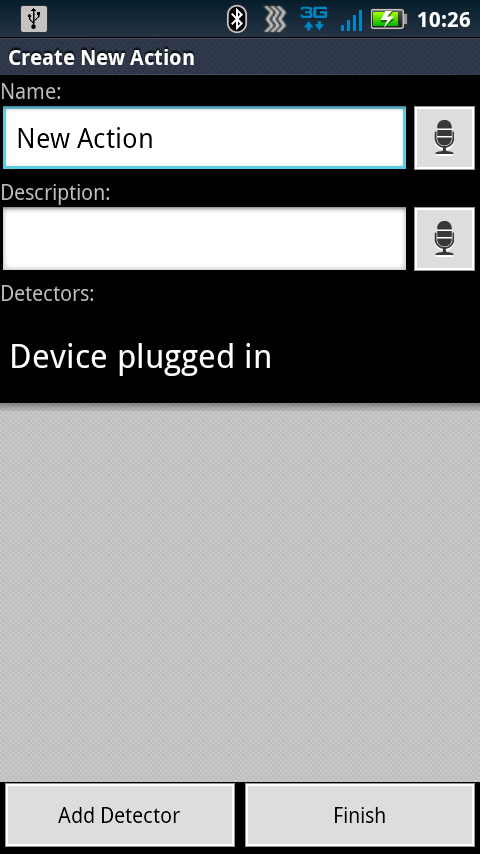
\includegraphics[height=2.5in]{voiceinput}
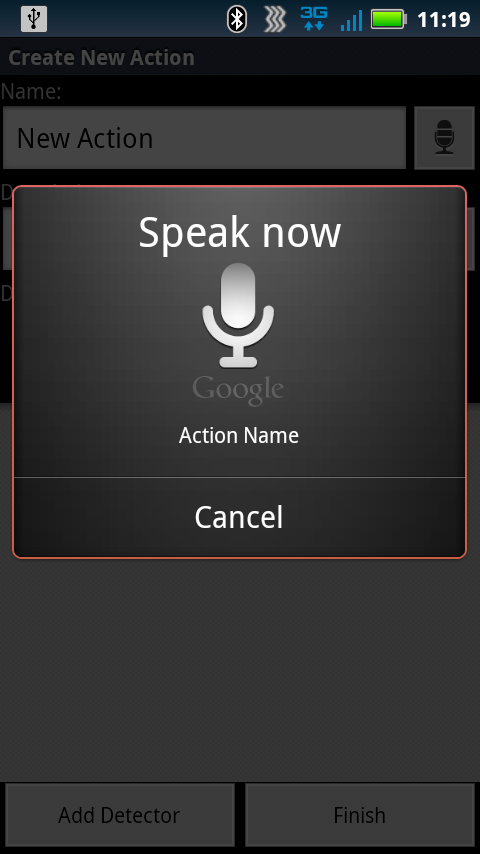
\includegraphics[height=2.5in]{voiceinput2}
\caption{
Creating a new action. All text fields are extended with a voice input button with a microphone icon.
}
\label{figure:voice}
\end{center}
\end{figure}


%%%%%%%%%%%%%%%%%%%%%%%%%%%%%%%%%%%%%%%%%%%%%%%%%%%%%%%%%%%%%%%

\section{Results and Assessment}
Results...
Assessment...

%%%%%%%%%%%%%%%%%%%%%%%%%%%%%%%%%%%%%%%%%%%%%%%%%%%%%%%%%%%%%%%

\section{Conclusions}
Conclusion...

%%%%%%%%%%%%%%%%%%%%%%%%%%%%%%%%%%%%%%%%%%%%%%%%%%%%%%%%%%%%%%%

\bibliographystyle{abbrv}
\bibliography{bibliography}  % sigproc.bib is the name of the Bibliography in this case

% That's all folks!
\end{document}
